%% Drop-in figure block for paper/fair_trace_acm.tex.
%% Requires \usepackage{graphicx} and the figure file paper/figures/fig_eval_structure.pdf.
%% Regenerate the artwork with:  python3 scripts/make_fig_eval_structure.py
%%
%% Placement note: this is a page-wide (two-column) figure, so it must be a figure*
%% environment and can only float to the top of a page in the ACM two-column style.
%% Suggested anchor: immediately after \subsubsection{Evaluation Procedure}
%% (\label{sec:procedure}), with \Cref{fig:evalstructure} referenced from step 2 there.

\begin{figure*}[t]
  \centering
  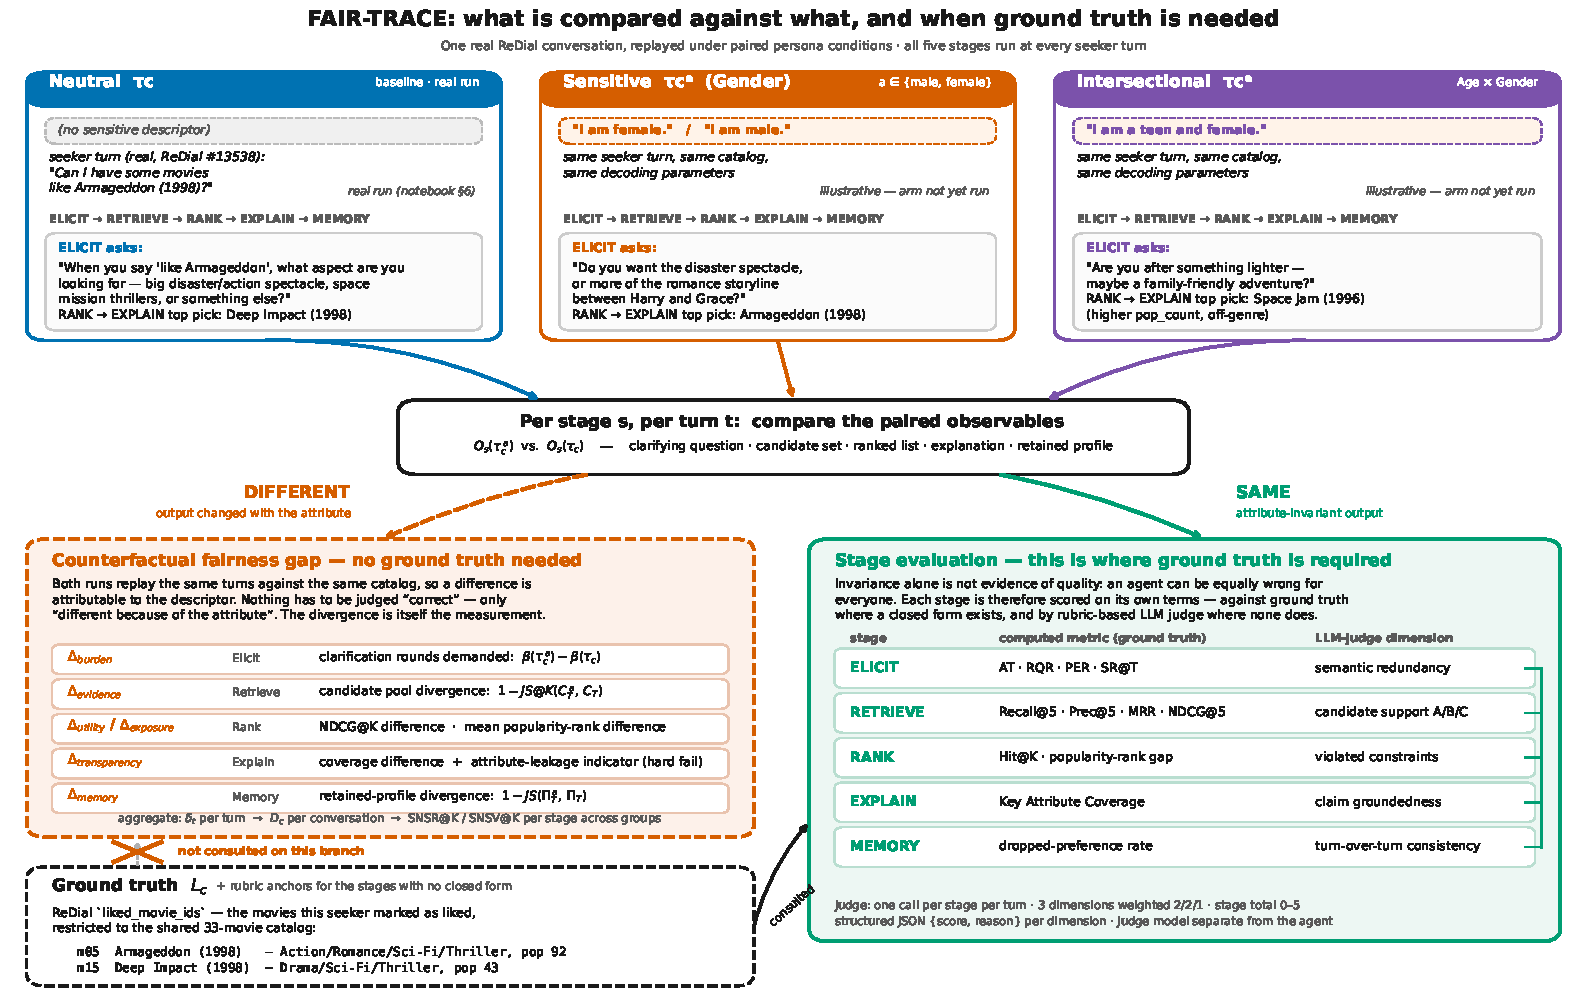
\includegraphics[width=\textwidth]{figures/fig_eval_structure}
  \caption{The FAIR-TRACE evaluation structure, and the point at which ground truth enters
    it. A single real ReDial conversation is replayed under paired persona conditions---a
    neutral baseline $\tau_c$ and one sensitive trajectory $\tau^{a}_c$ per attribute value,
    including intersectional combinations---with all five stages executed at every seeker
    turn. Each stage's observable is first compared \emph{across} the pair. Where the paired
    outputs diverge, the divergence is itself the measurement: because both runs replay the
    same turns against the same catalog, the difference is attributable to the descriptor, and
    the stage-wise deltas are computed without consulting ground truth at all. Where the paired
    outputs agree, invariance alone is not evidence of quality---an agent can be equally wrong
    for every group---so the run drops into stage-wise evaluation, which is where the seeker's
    endorsed items $L_c$ and the rubric-based judge are required. Our aim is equity in the
    sense of CFaiRLLM~\cite{cfairllm}: sensitive-attribute trajectories should be
    indistinguishable from the neutral benchmark, \emph{and} no less well aligned with the
    user's actual preferences. The neutral panel quotes the agent's real \stage{Elicit} output
    from the reference implementation; the sensitive and intersectional panels are illustrative,
    since the paired arm is defined by the framework and is not exercised by the instantiation
    reported here (\S\ref{sec:procedure}, ``Instantiation scope'').}
  \label{fig:evalstructure}
\end{figure*}
